%% Based on a TeXnicCenter-Template by Gyorgy SZEIDL.
%%%%%%%%%%%%%%%%%%%%%%%%%%%%%%%%%%%%%%%%%%%%%%%%%%%%%%%%%%%%%

%----------------------------------------------------------
%
\documentclass[letterpaper,12pt,openany,reqno]{book}%
%
%----------------------------------------------------------
% This is a sample document for the standard LaTeX Book Class
% Class options
%       --  Body text point size:
%                        10pt (default), 11pt, 12pt
%       --  Paper size:  letterpaper (8.5x11 inch, default)
%                        a4paper, a5paper, b5paper,
%                        legalpaper, executivepaper
%       --  Orientation (portrait is the default):
%                        landscape
%       --  Printside:   oneside, twoside (default)
%       --  Quality:     final(default), draft
%       --  Title page:  titlepage, notitlepage
%       --  Columns:     onecolumn (default), twocolumn
%       --  Start chapter on left:
%                        openright(no, default), openany
%       --  Equation numbering (equation numbers on right is the default):
%                        leqno
%       --  Displayed equations (centered is the default):
%                        fleqn (flush left)
%       --  Open bibliography style (closed bibliography is the default):
%                        openbib
% For instance the command
%          \documentclass[a4paper,12pt,reqno]{book}
% ensures that the paper size is a4, fonts are typeset at the size 12p
% and the equation numbers are on the right side.
%
\usepackage{amsmath}%
\usepackage{amsfonts}%
\usepackage{amssymb}%
\usepackage{graphicx}
\usepackage{tikz}
\usetikzlibrary{shapes,arrows}
%----------------------------------------------------------
\newtheorem{theorem}{Theorem}
\newtheorem{acknowledgement}[theorem]{Acknowledgement}
\newtheorem{algorithm}[theorem]{Algorithm}
\newtheorem{axiom}[theorem]{Axiom}
\newtheorem{case}[theorem]{Case}
\newtheorem{claim}[theorem]{Claim}
\newtheorem{conclusion}[theorem]{Conclusion}
\newtheorem{condition}[theorem]{Condition}
\newtheorem{conjecture}[theorem]{Conjecture}
\newtheorem{corollary}[theorem]{Corollary}
\newtheorem{criterion}[theorem]{Criterion}
\newtheorem{definition}[theorem]{Definition}
\newtheorem{example}[theorem]{Example}
\newtheorem{exercise}[theorem]{Exercise}
\newtheorem{lemma}[theorem]{Lemma}
\newtheorem{notation}[theorem]{Notation}
\newtheorem{problem}[theorem]{Problem}
\newtheorem{proposition}[theorem]{Proposition}
\newtheorem{remark}[theorem]{Remark}
\newtheorem{solution}[theorem]{Solution}
\newtheorem{summary}[theorem]{Summary}
\newenvironment{proof}[1][Proof]{\textbf{#1.} }{\ \rule{0.5em}{0.5em}}
%----------------------------------------------------------
\begin{document}

\frontmatter
\title{A Very Simple Compiler Book}
\author{Philip W. Howard}
\date{2019}
\maketitle
\tableofcontents

\chapter{Preface}

Given the existence of other very good books suitable for a course on compilers, why did I choose to write another one? There are several reasons:
  
\begin{enumerate}
\item Most compilers books seem to be written from the perspective that the course is preparing students to actually write a production compiler. That is not the perspective of the compiler courses I've taught. While the students in my course write a complete compiler, I readily acknowledge that very few of my students will work on a compiler as part of their career (although some have). The value of the course has more to do with helping the students to become better developers than in preparing them for a particular field. I have found that this difference in perspective alters what material I find most suitable for the courses I teach. 
\item I find the price of most text books almost criminal. By writing my own text, I can make electronic copies freely available and make printed copies available for a reasonable price.
\end{enumerate}

\mainmatter

\part{Overview}
\chapter{Introduction}
\section{Why?}
The first question that many prospective compiler students have is, ``Why should I study compilers?'' The following answers come to mind:

\begin{enumerate}
\item They're cool. Why wouldn't you want to study compilers?
\item It gives you a chance to understand what your primary tool does. It would seem strange for a carpenter to not know what a hammer does, or to not know the trade-offs between a hammer and a nail gun. Granted, a carpenter doesn't need to know the physics of how these tools work, but they should have a general idea. 

Many software developers never consider their compilers. They have this large blob of software known as an ``IDE''. They type specialized text into their IDE and click various buttons, and if they are luck, they get a working program. My claim is that better programmers have a better understanding of their tools. This allows them to make better use of these tools, and thus better use of their time, and thus (sometimes) more of their employer's money.

\item It gives you a chance to manage a large code base. I've heard of undergraduate computer science students who graduate having never managed anything bigger than a two week lab. In my ten week compiler course, students write an entire compiler composed of tens of source files and thousands of lines of code. Design and implementation decisions made early have strong consequences later in the term. This is a valuable experience that every developer should have before they step into a job claiming they know what they're doing.

Another advantage of the large project is that it allows the introduction of testing techniques that are harder to make ``real'' in smaller environments.

\item Applied data structures. A compiler has a lot of data that needs to be managed. Many data structures present ``clean'' data structures, but real-life data-problems often aren't so clean. How about a cyclic tree that contains links to a stack of hash tables that in turn has links back to nodes of the tree? OK, if your tree is cyclic, you probably have a bug, but most data structures classes don't give you the opportunity to make (and then fix) such bugs. Having the opportunity to get buried in data is good for you.

\item Applied algorithms. I started to learn calculus in high school. I continued my learning of calculus in college. But I didn't really understand what a $dx$ was until I encountered them in my calculus based physics class. They were no longer merely symbols on a paper, they were now applied, and that's how I finally grasped what they really were. In the same sense, a compiler allows you to apply quite a number of algorithms (and data structures). In doing so, they should be more ``real''.

\item Performance considerations. Computers have gotten so fast, we rarely have to worry about performance (time or memory) considerations. Most compiler runs are also fast enough that the compiler's performance doesn't much matter. But given a compiler, you can compile something very big like the Linux Kernel. Performance now matters. Because of this, a compiler class gives the right to talk about performance considerations in a practical sense.

\end{enumerate}

\section{What is a compiler?}
Perhaps before asking, ``Why study compilers?'' it would have been best to establish what a compiler is. But most students, by the time they get to a compiler course, have already used compilers so they have some sense of what they are: The software that translates my source code into executable code. We need to be a bit more formal as well as a bit broader in our definition.

In the broadest sense, a compiler takes code as input and outputs an improved version of that code. For the compiler to be valid, it must follow two guiding principles:
\begin{emumerate}
\item The compiler must preserve the meaning of the original program.
\item The compiler must improve the code in some discernible way.
\end{enumerate}


%----------------------------------------------------------
\begin{figure}[hbt]
\centering
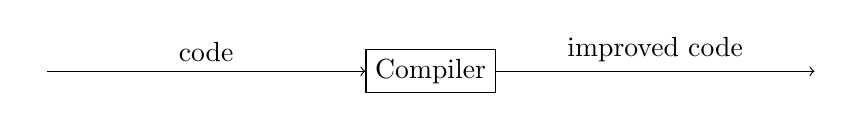
\begin{tikzpicture}
\node (a) at (-5,0) {};
\node (b) at (0,0) [shape=rectangle, draw] {Compiler};
\node (c) at (5,0) {};

\draw [->] (a) -- (b) node [midway, above] {code} ;
\draw [->] (b) -- (c) node [midway, above] {improved code} ;
%\draw [->] (b) -- (c) node [midway, above, text width=3cm, align=center] {improved\\code} ;
\end{tikzpicture}
 \caption[What is a Compiler]{A compiler is a program that takes code as input and outputs an improved version of that code.}
  \label{F.whatiscompiler}
\end{figure}
%----------------------------------------------------------

To illustrate the first principle, if you had a program that output the numbers from $1..10$ and the compiler transformed it so that it output one of e.e. cummings's poems, then clearly the compiler did not preserve the meaning of the original program.

The second principle is a bit less clear. If the code is a program, and you want to execute your program, then transforming your source code into an executable program would be an improvement. But suppose your source was a C program and the output was an equivalent Java program. Would that be an improvement?

This definition of a compiler is deliberately broad

\chapter{Compiler Structure}
Compilers are typically broken into two broad pieces: the front-end and the back-end. 
\chapter{Intermediate Representations}

\part{Scanning}

\chapter{Regular Expressions}

This chapter discusses regular expressions, what they are for, and how to use them.

\chapter{Creating a Scanner from Regular Expressions}

This chapter covers the algorithms for converting a list of Regular Expressions into code that can process them.

\section{Thompson's}

This section presents Thompson's construction.

\section{Subset Construction}

This section presents the Subset Construction

\chapter{Scanner Code}
\section{table driven}
Here is a table driven scanner
\section{switch statement}
Here is a table drive scanner

\chapter{Automatically Generated Scanners}
here is a description of flex.

\part{Parsing}
\chapter{Context Free Grammars}
\chapter {Top-down recursive-descent parsers}
\chapter {Bottom-up parsers}
\chapter {Automatically generated parsers}
Description of bison.

\part{The Back-end}
\chapter {The Visitor Pattern}
\chapter {Code generation}
\chapter {Optimization}

\subsubsection{Subsubsection}

This is just some text under a subsubsection.

\paragraph{Subsubsubsection}

This is just some  text under a subsubsubsection.

\subparagraph{Subsubsubsubsection}

This is just some text under a subsubsubsubsection.


\begin{itemize}
\item Bullet item 1

\item Bullet item 2

\end{itemize}

\begin{description}
\item[Description List] Each description list item has a term followed by the
description of that term.

\item[Bunyip] Mythical beast of Australian Aboriginal legends.
\end{description}

\section{Theorem-Like Environments}

The following theorem-like environments (in alphabetical order) are available
in this style.

\begin{acknowledgement}
This is an acknowledgement
\end{acknowledgement}

\begin{algorithm}
This is an algorithm
\end{algorithm}

\begin{axiom}
This is an axiom
\end{axiom}

\begin{case}
This is a case
\end{case}

\begin{claim}
This is a claim
\end{claim}

\begin{conclusion}
This is a conclusion
\end{conclusion}

\begin{condition}
This is a condition
\end{condition}

\begin{conjecture}
This is a conjecture
\end{conjecture}

\begin{corollary}
This is a corollary
\end{corollary}

\begin{criterion}
This is a criterion
\end{criterion}

\begin{definition}
This is a definition
\end{definition}

\begin{example}
This is an example
\end{example}

\begin{exercise}
This is an exercise
\end{exercise}

\begin{lemma}
This is a lemma
\end{lemma}

\begin{proof}
This is the proof of the lemma.
\end{proof}

\begin{notation}
This is notation
\end{notation}

\begin{problem}
This is a problem
\end{problem}

\begin{proposition}
This is a proposition
\end{proposition}

\begin{remark}
This is a remark
\end{remark}

\begin{summary}
This is a summary
\end{summary}

\begin{theorem}
This is a theorem
\end{theorem}

\begin{proof}
[Proof of the Main Theorem]This is the proof.
\end{proof}

\appendix

\chapter{The First Appendix}

The \verb"\appendix" command should be used only once. Subsequent appendices can
be created using the Chapter command.

\chapter{The Second Appendix}

Some text for the second Appendix.

This text is a sample for a short bibliography. You can cite a book by making use of
the command \verb"\cite{KarelRektorys}": \cite{KarelRektorys}. Papers can be cited
similarly: \cite{Bertoti97}. If you want multiple citations to appear in a single set
of square brackets you must type all of the citation keys inside a single citation,
separating each with a comma. Here is an example: \cite{Bertoti97, Szeidl2001,
Carlson67}.

\begin{thebibliography}{9}
\bibitem {KarelRektorys}Rektorys, K., \textit{Variational methods in Mathematics,
Science and Engineering}, D. Reidel Publishing Company,
Dordrecht-Hollanf/Boston-U.S.A., 2th edition, 1975

\bibitem {Bertoti97} \textsc{Bert\'{o}ti, E.}:\ \textit{On mixed variational formulation
of linear elasticity using nonsymmetric stresses and displacements}, International
Journal for Numerical Methods in Engineering., \textbf{42}, (1997), 561-578.

\bibitem {Szeidl2001} \textsc{Szeidl, G.}:\ \textit{Boundary integral equations for
plane problems in terms of stress functions of order one}, Journal of Computational and
Applied Mechanics, \textbf{2}(2), (2001), 237-261.

\bibitem {Carlson67}  \textsc{Carlson D. E.}:\ \textit{On G\"{u}nther's stress functions
for couple stresses}, Quart. Appl. Math., \textbf{25}, (1967), 139-146.
\end{thebibliography}

\backmatter

\chapter{Afterword}

The back matter often includes one or more of an index, an afterword,
acknowledgements, a bibliography, a colophon, or any other similar item. In
the back matter, chapters do not produce a chapter number, but they are
entered in the table of contents. If you are not using anything in the back
matter, you can delete the back matter TeX field and everything that follows it.
\end{document}
